
%!TEX root = 0卒業論文.tex
\newpage

\section{\rm 教材の構想}

\subsection{ビジュアルプログラミング}
本研究では,ビジュアルプログラミングを採用している.ビジュアルプログラミングとは,プログラムをテキストで記述するのではなく,視覚的に捉えやすいブロックなどをつなぎ合わせてプログラムを構築する.代表的なものでは,Scratchが存在しており,小学校プログラミング教育の実験授業などにも採用されている.
本研究で制作したサイトではScratchを採用している.

\subsection{本教材で目指すもの}
「Scratch」を用いて, 文部科学省が提唱した「プログラミング的思考」を構成する「自らの意図を明確化させる思考力」「どのような動きをどのような順序でさせれば良いのかを考える思考力」「どのように組み合わせれば良いかを考える思考力」を育成することを目的とし, 例題を提供する課題集サイトの作成である.

\subsection{全体の構成}
全体の構成は大きく3つに分け,「トップページ部」,「問題部」,「解説部」から構成した.
サイトの流れを図\ref{fig:nagare}に示す.

\begin{figure}[h]
\begin{center}
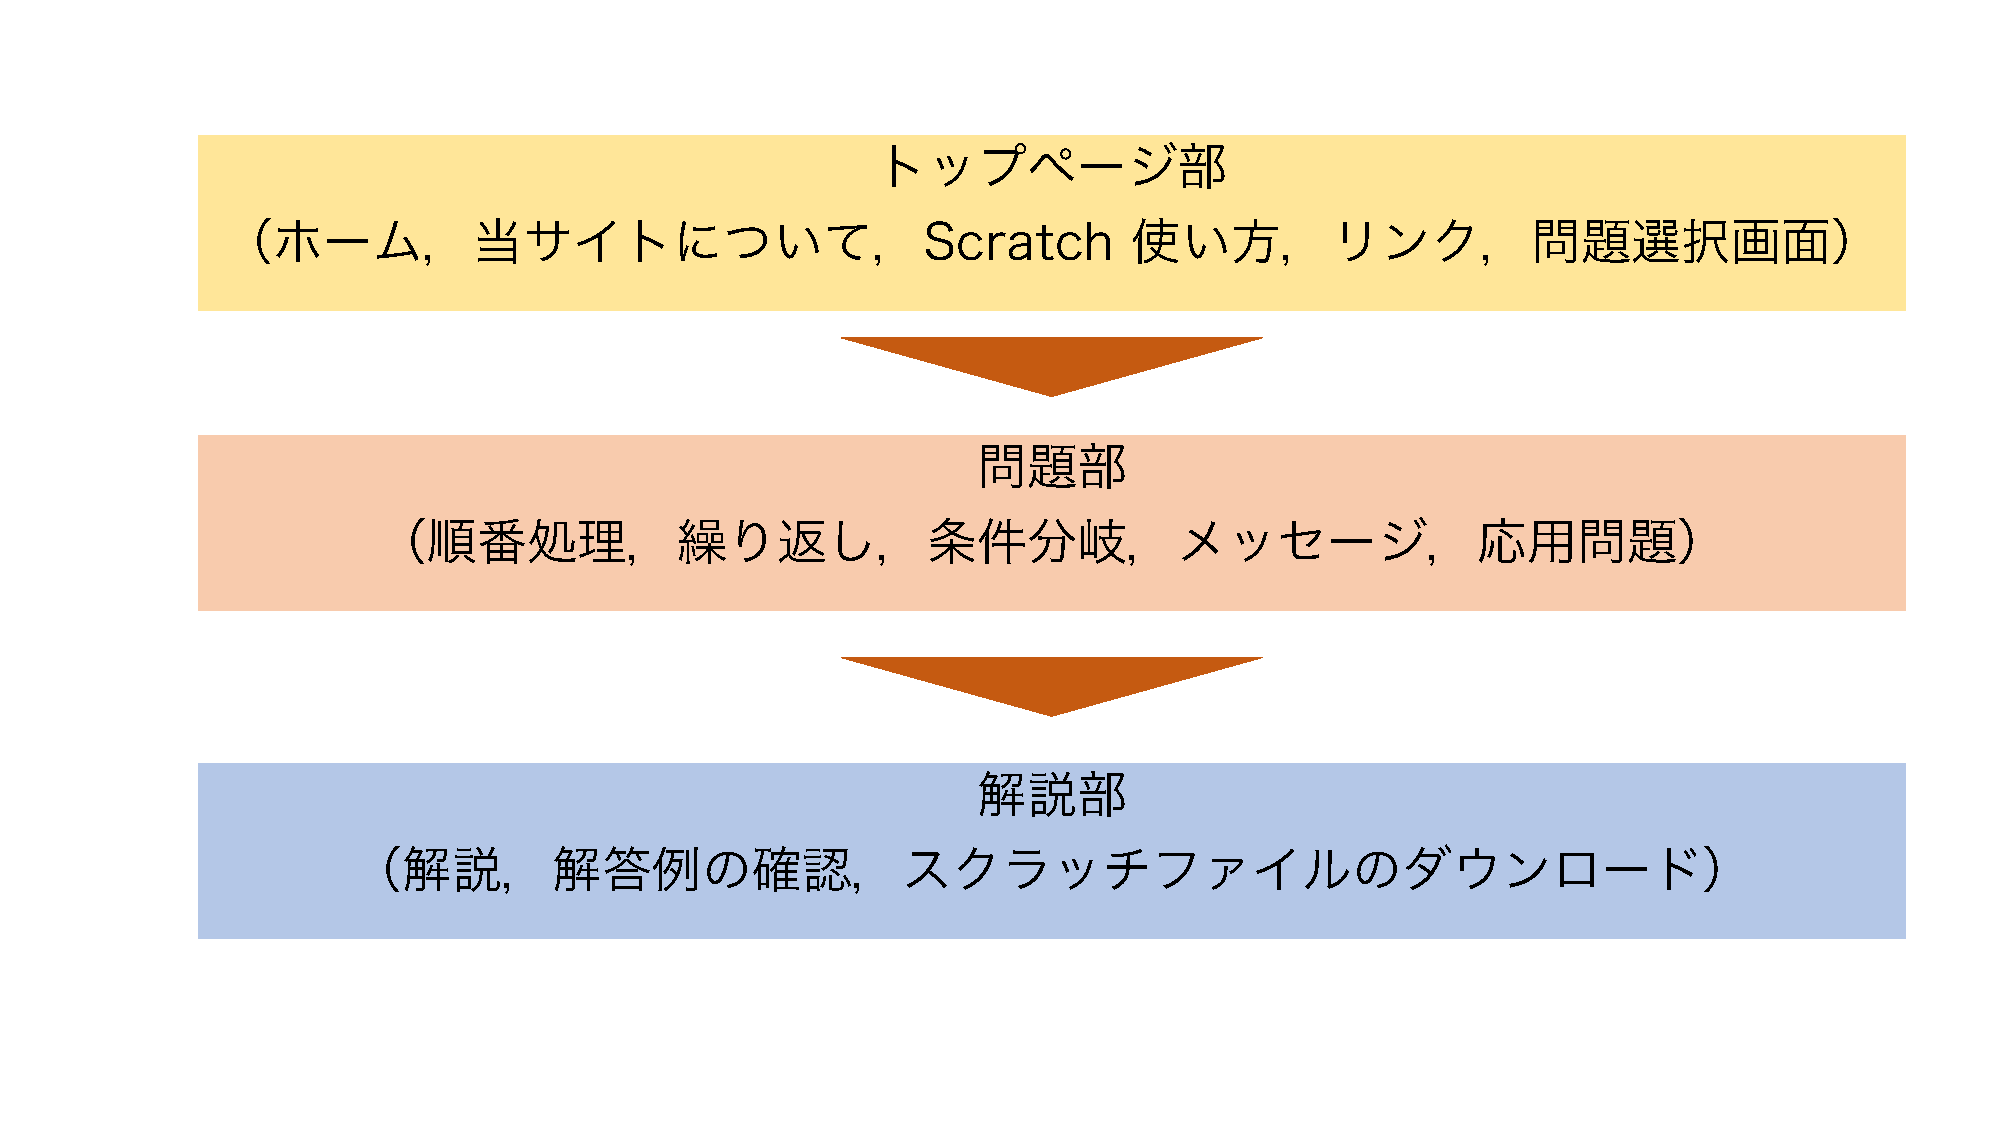
\includegraphics[width=15cm]{nagare.pdf}
\caption{サイト全体の流れ}
\label{fig:nagare}
\end{center}
\end{figure}
\newpage

\subsubsection{トップページ部}
課題集サイトのトップページ部分である.本サイトではホーム,当サイトについて,Scratch 使い方,問題選択画面,リンクから構成した.

\subsubsection{問題部}
サイト内で問題を出す部分である.問題は基本問題と応用問題から構成した.基本問題は「順番処理」,「繰り返し」,「条件分岐」,「メッセージ」の4つで構成した.

応用問題は基本問題を組み合わせて作成した発展的な問題である.

基本問題でのねらいを\ref{tab:nerai}に示す.
\begin{table}[htb]
\begin{center}
    \caption{トップページ部構成説明}
  \begin{tabular}{|c|c|} \hline
     処理名  & ねらい  \\ \hline
     順番処理& プログラムは上から下へ順に処理されていくこと \\ \hline
     繰り返し& 決まった回数や条件を満たすまで同じ処理を繰り返し行う \\ \hline
     条件分岐& 条件に応じて実行内容を切り替える \\ \hline
     メッセージ& 「〜を送る」と「〜を受け取ったとき」ブロックをセットで使いメッセージ処理を理解する \\ \hline
  \end{tabular}
  \label{tab:nerai}
  \end{center}
\end{table}
\subsubsection{解説部}
問題の解説部分である.問題の解答例,解説,スクラッチファイルのダウンロードを行うことができる.
\newpage

\subsection{基本問題部}
例として順番処理の問題を図\ref{fig:kihonrei}に示す.取り組んでもらう内容としては猫を10歩右に歩かせつつ大きさを50ずつ変えることである.
Scratchを用いてブロックを組み合わせ,課題を制作してもらうものとする.


\begin{figure}[h]
\begin{center}
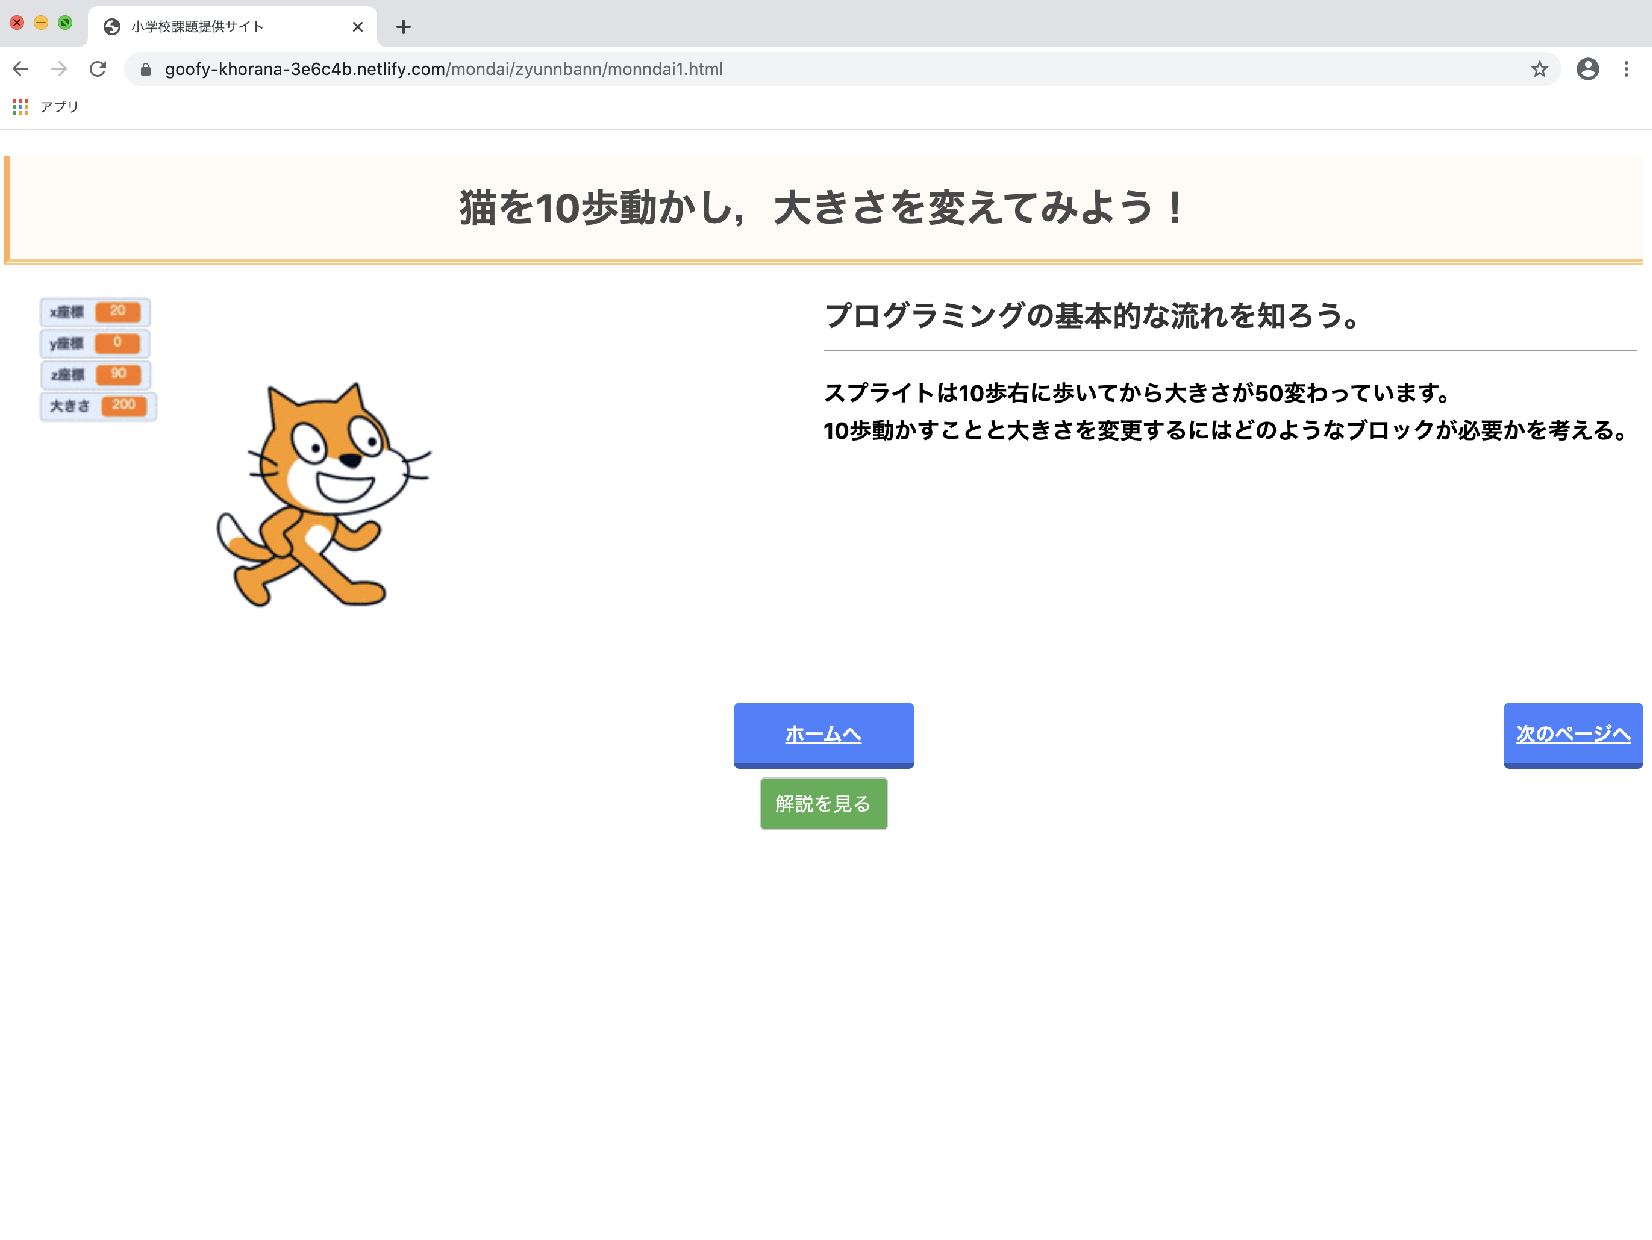
\includegraphics[width=15cm]{zyunnbanntoi.pdf}
\caption{基本問題 例}
\label{fig:kihonrei}
\end{center}
\end{figure}

\newpage

\subsubsection{基本問題部解説}
図\ref{fig:kihonreik}では「10歩動かす」命令と「大きさを50ずつ変える」の2つ命令を組み合わせることで,順番処理の基本である,上から下に処理していくことを学ぶことができる.

\begin{figure}[h]
\begin{center}
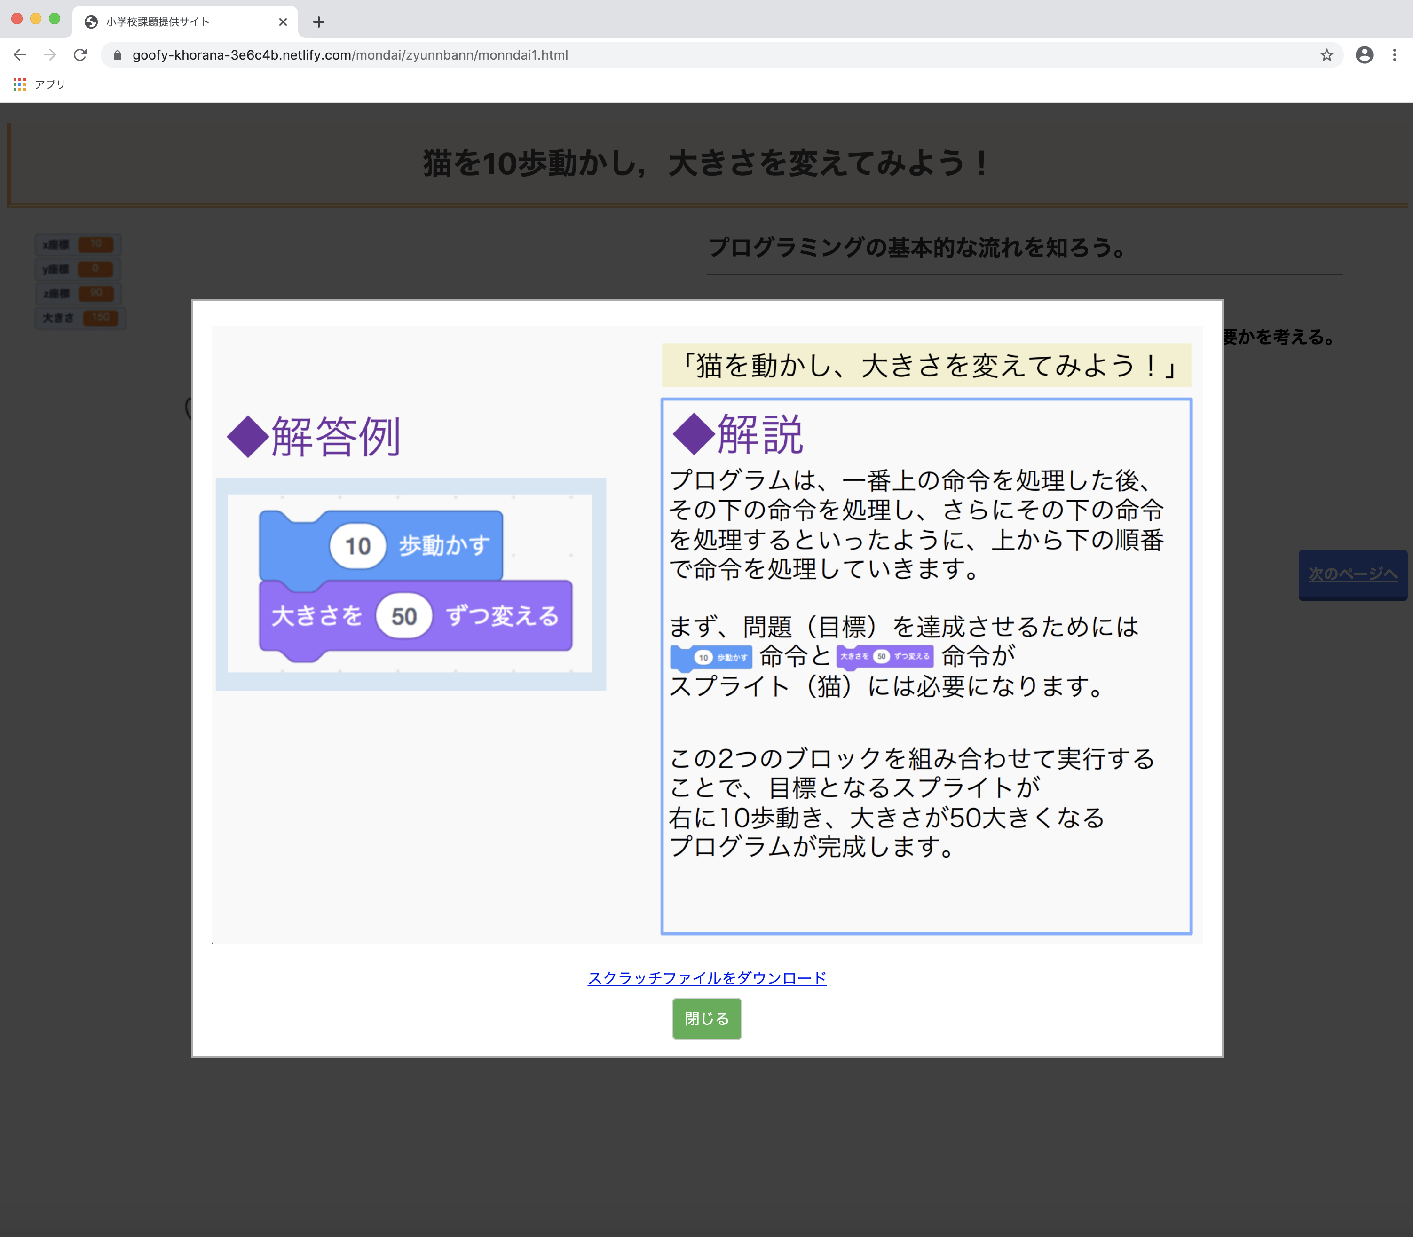
\includegraphics[width=15cm]{zyunnbannkotae.pdf}
\caption{基本問題部 解説 例}
\label{fig:kihonreik}
\end{center}
\end{figure}
\newpage

\subsection{応用問題部}
応用問題部の例として図\ref{fig:ouyou}に示す.
スプライトに問題を2つ問い,その答えをメッセージボックスに入力してもらう.
正解であれば「正解!」と2秒言い,不正解であれば「不正解!」と2秒言う.
2問答えた後に正解数に応じてスプライトが発言する内容が変わるプログラムである.



\begin{figure}[h]
\begin{center}
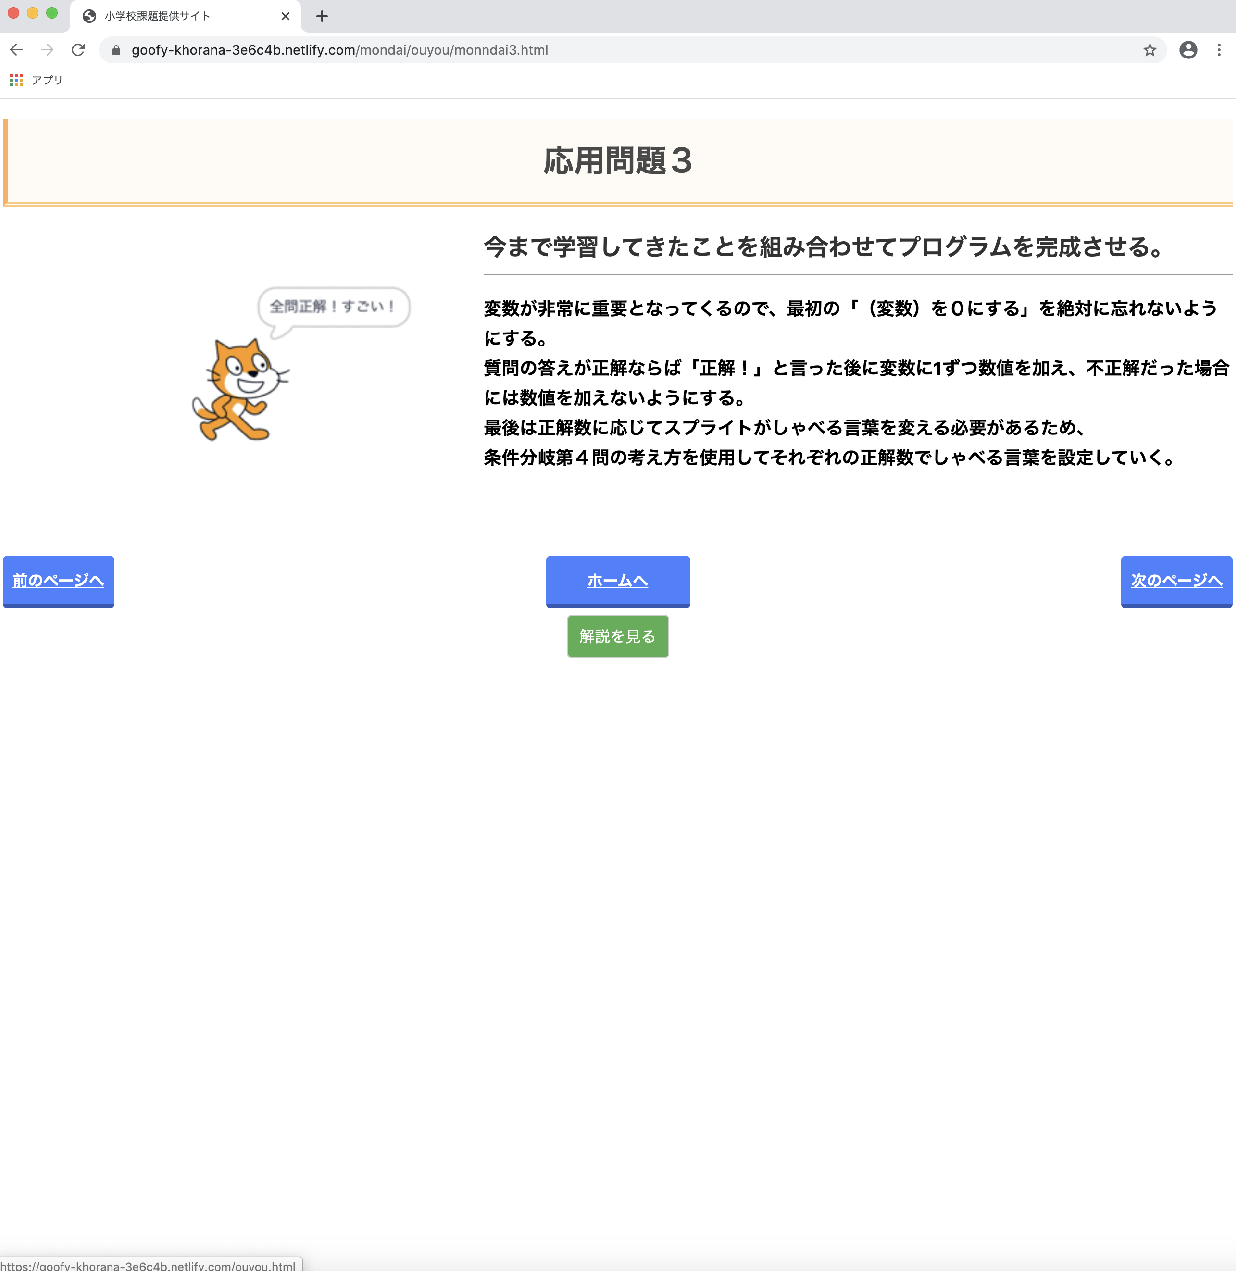
\includegraphics[width=15cm]{ouyoutoi.pdf}
\caption{応用問題部 例}
\label{fig:ouyou}
\end{center}
\end{figure}

\newpage

\subsubsection{応用問題部解説}
図\ref{fig:ouyouk}では正解数に応じてスプライトが発言する内容が変わることが重要である.そのため,スプライトが問題を正解した場合には変数を1変え,不正解の場合には変数を変えないといった処理が必要になる.




\begin{figure}[h]
\begin{center}
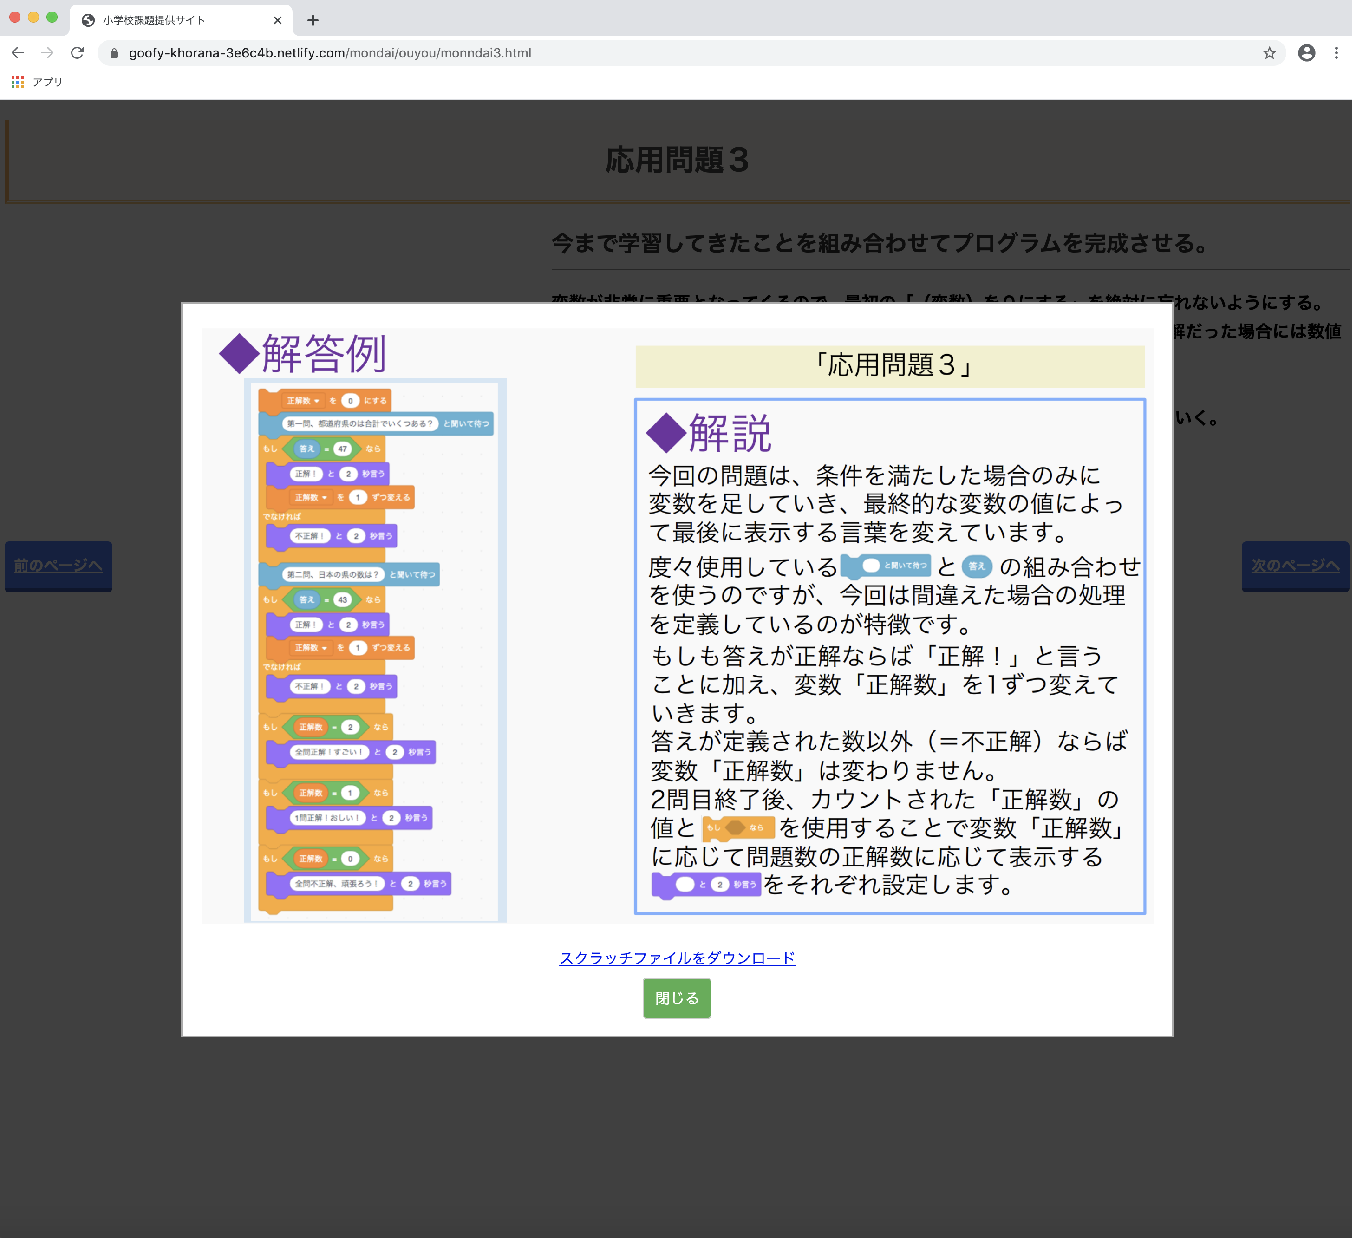
\includegraphics[width=15cm]{ouyoukotae.pdf}
\caption{応用問題部 解説 例}
\label{fig:ouyouk}
\end{center}
\end{figure}

